\chapter{Conjugate Gradient Methods}

In this chapter, we present the \emph{conjugate gradient methods},
which constitute a family of very efficient algorithms for solving
high-dimensional quadratic problems, as well as their
nonlinear extensions.

Conjugate gradient methods were introduced in the
1950s by Hestenes and Stiefel \cite{hestenes1952methods} to solve linear systems
\[
A x = b,
\]
where $A \in \R^{n \times n}$ is symmetric positive definite. Later,
Fletcher and Reeves \cite{fletcher1964function} proposed a \emph{nonlinear} extension for
the minimization of a general function $f : \R^n \to \R$.

\medskip

Compared to gradient descent:
\begin{itemize}
  \item they do not require storing the matrix $A$;
  \item they converge much faster on well-conditioned quadratic problems;
  \item they are particularly suitable for high dimensions.
\end{itemize}

%%%%%%%%%%%%%%%%%%%%%%%%%%%%%%%%%%%%%%%%%%%%%%%%%%%%%%%%%%%%
\section{Linear Conjugate Gradient}

\subsection{Associated Quadratic Problem}

Consider the linear system
\[
A x = b,
\]
where $A$ is symmetric positive definite. This problem is equivalent to minimizing
\begin{equation}
q(x) = \frac{1}{2} x^\top A x - b^\top x.
\label{eq:cg-quadratic}
\end{equation}
Its gradient is
\[
\nabla q(x) = A x - b,
\]
and thus $x^\star$ minimizes $q$ if and only if $A x^\star = b$.

For a direction $p_k$, we minimize $q(x_k + \alpha p_k)$:
\[
\psi(\alpha) = q(x_k + \alpha p_k).
\]
The condition $\psi'(\alpha)=0$ gives
\[
p_k^\top A (x_k + \alpha p_k) - p_k^\top b = 0.
\]
Since $r_k = A x_k - b$:
\[
\boxed{\alpha_k = -\frac{p_k^\top r_k}{p_k^\top A p_k}}.
\]

%%%%%%%%%%%%%%%%%%%%%%%%%%%%%%%%%%%%%%%%%%%%%%%%%%%%%%%%%%%%
\subsection{\texorpdfstring{$A$}{A}-Conjugate Directions}

\begin{definition}
Two non-zero vectors $p_i,p_j$ are \emph{$A$-conjugate} if
\[
p_i^\top A p_j = 0.
\]
A family $(p_0,\dots,p_m)$ is $A$-conjugate if all its distinct vectors are pairwise $A$-conjugate.
\end{definition}

An $A$-conjugate family forms a basis in which the minimization becomes independent between components: a correction in one direction does not degrade the ones already made.

%%%%%%%%%%%%%%%%%%%%%%%%%%%%%%%%%%%%%%%%%%%%%%%%%%%%%%%%%%%%
\subsection{Conjugate Direction Method}

Assume we are given $A$-conjugate directions $(\eta_0,\dots,\eta_{n-1})$. We set:
\[
x_{k+1} = x_k + \alpha_k \eta_k, \qquad
\alpha_k = -\frac{\eta_k^\top r_k}{\eta_k^\top A \eta_k}.
\]

\begin{theoreme}[Minimization over expanding subspaces]
For $k \ge 1$:
\[
r_k^\top \eta_i = 0 \quad (i<k),
\]
and
\[
\boxed{x_k = \arg\min_{x \in x_0 + \mathrm{span}(\eta_0,\dots,\eta_{k-1})} q(x)}.
\]
\end{theoreme}

%%%%%%%%%%%%%%%%%%%%%%%%%%%%%%%%%%%%%%%%%%%%%%%%%%%%%%%%%%%%
\subsection{Linear Conjugate Gradient Algorithm}

We denote $r_k = A x_k - b$.

We define the directions by
\[
p_0 = -r_0,\qquad p_k = -r_k + \beta_k p_{k-1}.
\]
The $A$-conjugacy condition $p_k^\top A p_{k-1}=0$ requires
\[
\boxed{\beta_k = \frac{r_k^\top A p_{k-1}}{p_{k-1}^\top A p_{k-1}}}
\quad\text{(Linear Hestenes–Stiefel \cite{hestenes1952methods}).}
\]
In practice, one often uses the equivalent form
\[
\beta_k = \frac{r_k^\top r_k}{r_{k-1}^\top r_{k-1}}.
\]

\begin{algorithm}[H]
\caption{Preliminary Version of Conjugate Gradient}
\label{alg:cg-preliminary}
Given $x_0$\;
Set $r_0 \leftarrow Ax_0 - b$, $p_0 \leftarrow -r_0$, $k \leftarrow 0$\;
\While{$r_k \neq 0$}{
    $\alpha_k \leftarrow -\dfrac{r_k'p_k}{p_k'Ap_k}$\;
    $x_{k+1} \leftarrow x_k + \alpha_k p_k$\;
    $r_{k+1} \leftarrow Ax_{k+1} - b$\;
    $\beta_{k+1} \leftarrow \dfrac{r_{k+1}'Ap_k}{p_k'Ap_k}$\;
    $p_{k+1} \leftarrow -r_{k+1} + \beta_{k+1}p_k$\;
    $k \leftarrow k + 1$\;
}
\end{algorithm}

\begin{algorithm}[H]
\caption{Conjugate Gradient (practical version)}
\label{alg:cg-practical}
Given $x_0$\;
Set $r_0 \leftarrow Ax_0 - b$, $p_0 \leftarrow -r_0$, $k \leftarrow 0$\;
\While{$r_k \neq 0$}{
    $\alpha_k \leftarrow \dfrac{r_k'r_k}{p_k'Ap_k}$\;
    $x_{k+1} \leftarrow x_k + \alpha_k p_k$\;
    $r_{k+1} \leftarrow r_k + \alpha_k Ap_k$\;
    $\beta_{k+1} \leftarrow \dfrac{r_{k+1}'r_{k+1}}{r_k'r_k}$\;
    $p_{k+1} \leftarrow -r_{k+1} + \beta_{k+1}p_k$\;
    $k \leftarrow k + 1$\;
}
\end{algorithm}

\begin{remarque}
The practical version avoids recalculating $Ax_{k+1}$ by using the recurrence relation $r_{k+1} = r_k + \alpha_k Ap_k$.
Furthermore, the formulas for $\alpha_k$ and $\beta_{k+1}$ only require inner products.
\end{remarque}

The following properties hold:
\[
r_i^\top r_j = 0, \qquad p_i^\top A p_j = 0 \quad(i\neq j).
\]

%%%%%%%%%%%%%%%%%%%%%%%%%%%%%%%%%%%%%%%%%%%%%%%%%%%%%%%%%%%%
\subsection{Error Bound and Conditioning}

If $\lambda_{\min}$ and $\lambda_{\max}$ are the extreme eigenvalues of $A$, then
\[
\frac{\|x_k - x^\star\|_A}{\|x_0 - x^\star\|_A}
\le
2\left(\frac{\sqrt{\kappa(A)} - 1}{\sqrt{\kappa(A)} + 1}\right)^k,
\qquad
\kappa(A)=\frac{\lambda_{\max}}{\lambda_{\min}}.
\]

%%%%%%%%%%%%%%%%%%%%%%%%%%%%%%%%%%%%%%%%%%%%%%%%%%%%%%%%%%%%
\section{Geometric Interpretation}

\subsection{Level sets of a quadratic function}

The level sets of \eqref{eq:cg-quadratic} are ellipses centered at $x^\star$.  
The conjugate gradient follows successively $A$-conjugate directions, which allows "correcting" the error in each direction independently.

\begin{figure}[H]
  \centering
  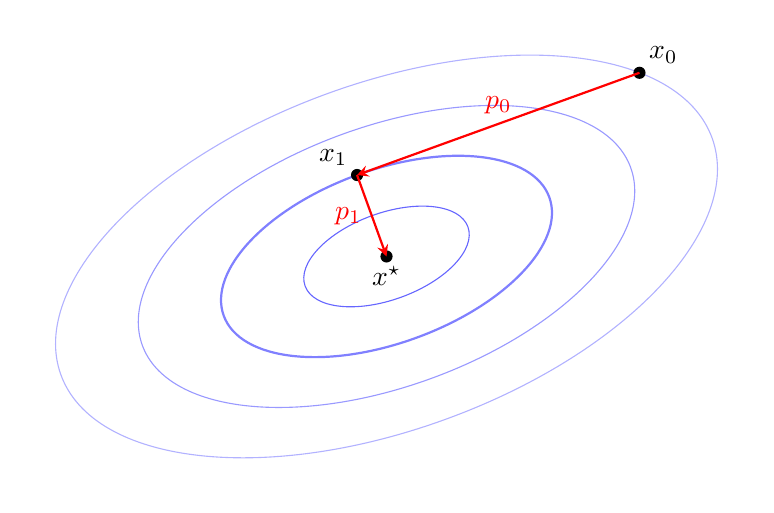
\begin{tikzpicture}[scale=1.1, >=stealth]
    \coordinate (xstar) at (0,0);
    % Level sets (ellipses) - tilted by 20 degrees for consistency with p0 direction
    \begin{scope}[rotate=20]
      \draw[blue!30]       (0,0) ellipse (4 and 2);
      \draw[blue!40]       (0,0) ellipse (3 and 1.5);
      \draw[thick,blue!50] (0,0) ellipse (2 and 1);
      \draw[blue!60]       (0,0) ellipse (1 and 0.5);
    \end{scope}
    
    % x1 on ellipse (2,1) at top of minor axis (s=90°)
    % x = -1*sin(20°) = -0.34, y = 1*cos(20°) = 0.94
    % p1 from x1 to x* will be along minor axis
    \coordinate (x1) at (-0.34, 0.94);
    \fill (x1) circle (2pt) node[above left] {$x_1$};
    
    % x0 on outer ellipse (4,2) at t=30°, positioned so p0 is parallel to major axis
    % x = 4*cos(30°)*cos(20°) - 2*sin(30°)*sin(20°) = 2.92
    % y = 4*cos(30°)*sin(20°) + 2*sin(30°)*cos(20°) = 2.12
    % Direction to x1: slope = 1.18/3.26 ≈ 0.36 = tan(20°) ✓
    \coordinate (x0) at (2.92, 2.12);
    \fill (x0) circle (2pt) node[above right] {$x_0$};
    
    % x* at center
    \fill (xstar) circle (2pt) node[below] {$x^\star$};
    
    % Direction p0: from x0 to x1 - parallel to major axis (slope = tan(20°))
    \draw[->, thick, red] (x0) -- (x1) node[midway, above] {$p_0$};
    
    % Direction p1: from x1 to x* - along minor axis
    \draw[->, thick, red] (x1) -- (xstar) node[midway, left] {$p_1$};
  \end{tikzpicture}
  \caption{Geometric interpretation: level sets of $q$ and conjugate directions.}
\end{figure}

In two dimensions, the conjugate gradient reaches exactly $x^\star$ in two iterations.

%%%%%%%%%%%%%%%%%%%%%%%%%%%%%%%%%%%%%%%%%%%%%%%%%%%%%%%%%%%%
\section{Comparison with Gradient Descent}

Gradient descent zigzags on elongated ellipses, while the conjugate gradient chooses directions that will progressively "diagonalize" the matrix $A$.

%%%%%%%%%%%%%%%%%%%%%%%%%%%%%%%%%%%%%%%%%%%%%%%%%%%%%%%%%%%%
\section{Preconditioning}

When $A$ is ill-conditioned, we introduce an SPD matrix $M$
approximating $A$ or $A^{-1}$.  
We consider the equivalent system:
\[
M^{-1} A x = M^{-1} b.
\]

We introduce $z_k = M^{-1} r_k$.

\begin{algorithm}[H]
\caption{Preconditioned Conjugate Gradient}
\label{alg:pcg}
Given $x_0$, preconditioner $M$\;
Set $r_0 \leftarrow Ax_0 - b$\;
Solve $My_0 = r_0$ for $y_0$\;
Set $p_0 \leftarrow -y_0$, $k \leftarrow 0$\;
\While{$r_k \neq 0$}{
    $\alpha_k \leftarrow \dfrac{r_k'y_k}{p_k'Ap_k}$\;
    $x_{k+1} \leftarrow x_k + \alpha_k p_k$\;
    $r_{k+1} \leftarrow r_k + \alpha_k Ap_k$\;
    Solve $My_{k+1} = r_{k+1}$\;
    $\beta_{k+1} \leftarrow \dfrac{r_{k+1}'y_{k+1}}{r_k'y_k}$\;
    $p_{k+1} \leftarrow -y_{k+1} + \beta_{k+1}p_k$\;
    $k \leftarrow k + 1$\;
}
\end{algorithm}
%%%%%%%%%%%%%%%%%%%%%%%%%%%%%%%%%%%%%%%%%%%%%%%%%%%%%%%%%%%%
\section{Nonlinear Conjugate Gradient}

We seek to minimize $f(x)$, assumed to be $\mathcal{C}^1$.  
Let $g_k = \nabla f(x_k)$.

\begin{algorithm}[H]
\caption{Fletcher-Reeves Method}
\label{alg:fletcher-reeves}
Given $x_0$\;
Evaluate $f_0 = f(x_0)$, $\nabla f_0 = \nabla f(x_0)$\;
Set $p_0 = -\nabla f_0$, $k \leftarrow 0$\;
\While{$\nabla f_k \neq 0$}{
    Compute $\alpha_k$ and set $x_{k+1} = x_k + \alpha_k p_k$\;
    Evaluate $\nabla f_{k+1}$\;
    $\beta_{k+1}^{FR} \leftarrow \dfrac{\nabla f_{k+1}'\nabla f_{k+1}}{\nabla f_k'\nabla f_k}$\;
    $p_{k+1} \leftarrow -\nabla f_{k+1} + \beta_{k+1}^{FR}p_k$\;
    $k \leftarrow k + 1$\;
}
\end{algorithm}

\begin{theoreme}
If the line search satisfies the Wolfe conditions and $f$ is smooth, then
\[
\liminf_{k\to\infty} \|g_k\| = 0.
\]
\end{theoreme}

%%%%%%%%%%%%%%%%%%%%%%%%%%%%%%%%%%%%%%%%%%%%%%%%%%%%%%%%%%%%
\section{Summary}

\begin{itemize}
  \item The linear conjugate gradient is optimal for SPD quadratic problems.
  \item Directions are $A$-conjugate and residuals orthogonal.
  \item Preconditioning drastically improves convergence.
  \item The nonlinear conjugate gradient is efficient and inexpensive.
  \item The choice of $\beta_k$ strongly influences performance.
\end{itemize}

%%%%%%%%%%%%%%%%%%%%%%%%%%%%%%%%%%%%%%%%%%%%%%%%%%%%%%%%%%%%
\subsection{Properties of Iterates and Krylov Subspaces}

The following properties justify the theoretical efficiency of the method.

\begin{theoreme}
Suppose that the $k$-th iterate is not equal to the solution $x^\star$. Then:
\begin{enumerate}
    \item[(i)] The residuals are orthogonal:
    \[ \forall i = 0, \dots, k-1, \quad r_k^\top r_i = 0. \]
    
    \item[(ii)] The space spanned by the residuals is a Krylov subspace of degree $k$ for $r_0$:
    \[ \mathrm{span}(r_0, \dots, r_k) = \mathrm{span}(r_0, A r_0, \dots, A^k r_0). \]
    
    \item[(iii)] The space spanned by the descent directions coincides with this space:
    \[ \mathrm{span}(p_0, \dots, p_k) = \mathrm{span}(r_0, A r_0, \dots, A^k r_0). \]
    
    \item[(iv)] The directions are $A$-conjugate to the previous ones:
    \[ \forall i = 0, \dots, k-1, \quad p_k^\top A p_i = 0. \]
\end{enumerate}
\end{theoreme}

\begin{proof}[Proof]
Reference: \cite{nocedal2006numerical}.
\end{proof}

\paragraph{Consequences.}
From point (iv), the conjugate gradient converges to $x^\star$ in at most $n$ iterations (in exact arithmetic), since there can be no more than $n$ mutually $A$-conjugate non-zero directions in $\R^n$.

\begin{remarque}
It is essential for these properties that the initialization is $p_0 = -r_0 = -(A x_0 - b)$.
\end{remarque}

%%%%%%%%%%%%%%%%%%%%%%%%%%%%%%%%%%%%%%%%%%%%%%%%%%%%%%%%%%%%
\subsection{Derivation of the efficient version (Standard CG)}
\label{sec:efficient-cg}

Up to now, we had the general formula for $\alpha_k$. We can simplify it to reduce the computational cost.

We know that:
\[ \alpha_k = \frac{-r_k^\top p_k}{p_k^\top A p_k}. \]
According to the expanding subspace minimization (ESM) theorem, we know that $r_k^\top p_i = 0$ for all $i = 0, \dots, k-1$.
Since $p_k = -r_k + \beta_k p_{k-1}$, we have:
\[ 
-r_k^\top p_k = -r_k^\top (-r_k + \beta_k p_{k-1}) = r_k^\top r_k - \beta_k \underbrace{r_k^\top p_{k-1}}_{=0}.
\]
Thus, the simplified formula for the step is:
\[
\boxed{\alpha_k = \frac{r_k^\top r_k}{p_k^\top A p_k}}.
\]

Next, for the coefficient $\beta_{k+1}$, we start from the definition ensuring $A$-conjugacy:
\[
\beta_{k+1} = \frac{r_{k+1}^\top A p_k}{p_k^\top A p_k}.
\]
We use the residual recurrence relation: $r_{k+1} = r_k + \alpha_k A p_k$, which implies $A p_k = \frac{1}{\alpha_k}(r_{k+1} - r_k)$.

Substituting into the numerator:
\[
r_{k+1}^\top A p_k = \frac{1}{\alpha_k} r_{k+1}^\top (r_{k+1} - r_k) = \frac{1}{\alpha_k} (r_{k+1}^\top r_{k+1} - \underbrace{r_{k+1}^\top r_k}_{=0}) = \frac{r_{k+1}^\top r_{k+1}}{\alpha_k}.
\]
Similarly for the denominator, we know that $p_k^\top A p_k = \frac{r_k^\top r_k}{\alpha_k}$.

Thus, the ratio simplifies remarkably:
\[
\beta_{k+1} = \frac{\frac{r_{k+1}^\top r_{k+1}}{\alpha_k}}{\frac{r_k^\top r_k}{\alpha_k}} = \frac{r_{k+1}^\top r_{k+1}}{r_k^\top r_k}.
\]

\paragraph{Remarks on Algorithm 7 (Standard CG):}
\begin{itemize}
    \item We eliminated the matrix-vector products in calculating the scalar coefficients (they only remain in the update $Ap_k$).
    \item We only need to store the values of $x$, $p$, and $r$ over two iterations.
\end{itemize}

%%%%%%%%%%%%%%%%%%%%%%%%%%%%%%%%%%%%%%%%%%%%%%%%%%%%%%%%%%%%
\section{Rate of Convergence}

\begin{theoreme}[\cite{nocedal2006numerical}]
If the matrix $A$ has only $r$ distinct eigenvalues, then convergence occurs in at most $r$ iterations.
\end{theoreme}

A more precise error bound is given by the following theorem, which depends on the eigenvalue distribution.

\begin{theoreme}[\cite{luenberger1984linear}]
If $A$ has eigenvalues $\lambda_1 \le \dots \le \lambda_n$, then:
\[
\| x_{k+1} - x^\star \|_A^2 \le \left( \frac{\lambda_{n-k} - \lambda_1}{\lambda_{n-k} + \lambda_1} \right)^2 \| x_0 - x^\star \|_A^2.
\]
\end{theoreme}
This result suggests that the conjugate gradient eliminates the influence of the extreme eigenvalues as the iterations proceed.

%%%%%%%%%%%%%%%%%%%%%%%%%%%%%%%%%%%%%%%%%%%%%%%%%%%%%%%%%%%%
\subsection{Illustration: Effect of eigenvalue distribution}

Consider a matrix $A$ having 2 "clusters" of eigenvalues:
\begin{itemize}
    \item A large group of $n-m$ eigenvalues close to $\lambda_1$.
    \item A small group of $m$ eigenvalues (outliers) located further away.
\end{itemize}

According to Luenberger's theorem, after $m$ iterations, we eliminate the influence of the $m$ extreme eigenvalues. The error at step $m+1$ then satisfies:
\[
\|x_{m+1} - x^\star\|_A^2 \le \left( \frac{\lambda_{n-m} - \lambda_1}{\lambda_{n-m} + \lambda_1} \right)^2 \|x_0 - x^\star\|_A^2.
\]
Roughly speaking, this means effective convergence starts after dealing with the few isolated eigenvalues.

%%%%%%%%%%%%%%%%%%%%%%%%%%%%%%%%%%%%%%%%%%%%%%%%%%%%%%%%%%%%
\subsection{Comparison of convergence rates}

It is instructive to compare the error bound of Conjugate Gradient (CG) with that of the Steepest Descent (SD) method.

We denote the condition number $\kappa(A) = \|A\| \cdot \|A^{-1}\| = \frac{\lambda_n}{\lambda_1}$.

\begin{itemize}
    \item \textbf{For Conjugate Gradient (CG):}
    \[
    \|x_k - x^\star\|_A \le 2 \left( \frac{\sqrt{\kappa(A)} - 1}{\sqrt{\kappa(A)} + 1} \right)^k \|x_0 - x^\star\|_A.
    \]

    \item \textbf{For Steepest Descent (SD):}
    \[
    \|x_k - x^\star\|_A \le \left( \frac{\kappa(A) - 1}{\kappa(A) + 1} \right)^k \|x_0 - x^\star\|_A.
    \]
\end{itemize}

\begin{remarque}
When $\kappa(A)$ is large (ill-conditioned problem), the term $\frac{\kappa(A)-1}{\kappa(A)+1}$ is very close to 1, which implies a very slow convergence (numerical "zigzagging").
In contrast, the term with the square root $\sqrt{\kappa(A)}$ in CG is much more favorable, ensuring faster convergence.
\end{remarque}

%%%%%%%%%%%%%%%%%%%%%%%%%%%%%%%%%%%%%%%%%%%%%%%%%%%%%%%%%%%%
\section{Preconditioning}
\label{sec:preconditioning}

\subsection{General Idea}

The idea of preconditioning is to "transform" the eigenvalue distribution of $A$ to accelerate convergence.

We perform a change of variable from $x$ to $\hat{x}$:
\[
\hat{x} = C x \iff x = C^{-1} \hat{x},
\]
where $C$ is an invertible (non-singular) matrix.

The quadratic objective function $\phi(x)$ then becomes a function of $\hat{x}$, denoted $\hat{\phi}(\hat{x})$:
\[
\hat{\phi}(\hat{x}) = \phi(C^{-1}\hat{x}) = \frac{1}{2} (C^{-1}\hat{x})^\top A (C^{-1}\hat{x}) - b^\top (C^{-1}\hat{x}).
\]

Expanding, we obtain:
\[
\hat{\phi}(\hat{x}) = \frac{1}{2} \hat{x}^\top \left[ (C^{-1})^\top A C^{-1} \right] \hat{x} - \left( (C^{-1})^\top b \right)^\top \hat{x}.
\]

\subsection{Choosing the preconditioning matrix}

The function $\hat{\phi}$ is still quadratic. If we use the Conjugate Gradient to minimize $\hat{\phi}$, performance will now depend on the eigenvalues of the new coefficient matrix:
\[
\hat{A} = (C^{-1})^\top A C^{-1}.
\]

We must therefore choose the matrix $C$ such that:
\begin{enumerate}
    \item The condition number of $(C^{-1})^\top A C^{-1}$ is lower than that of $A$ (i.e. $\kappa(\hat{A}) < \kappa(A)$).
    \item Or the eigenvalues of $(C^{-1})^\top A C^{-1}$ are well clustered.
\end{enumerate}

In practice, we do not explicitly build $\hat{A}$. We often set $M = C^\top C$ (the preconditioner) and adapt the CG algorithm to implicitly solve the system $M^{-1} A x = M^{-1} b$.

%%%%%%%%%%%%%%%%%%%%%%%%%%%%%%%%%%%%%%%%%%%%%%%%%%%%%%%%%%%%
\subsection{Practical Implementation}

In practice, we only need to use the matrix $C$ through the preconditioner $M$ defined by:
\[
M = C^\top C.
\]
This leads to Algorithm 8 (Preconditioned Conjugate Gradient).

\paragraph{Balance.}
The use of preconditioning implies a trade-off:
\begin{itemize}
    \item[(+)] Preconditioning improves the eigenvalue distribution (reducing the number of iterations).
    \item[(-)] It introduces linear system solves $M y = r$ at each step.
\end{itemize}
The goal is thus to choose $M$ so that the system $M y = r$ is inexpensive to solve.

%%%%%%%%%%%%%%%%%%%%%%%%%%%%%%%%%%%%%%%%%%%%%%%%%%%%%%%%%%%%
\subsection{Example: Incomplete Cholesky Preconditioning}

A classical method relies on the Cholesky decomposition. For a symmetric positive definite matrix $A$, there exists a lower triangular matrix $L$ such that $A = L L^\top$.

\textbf{Idea:} We seek an approximation of $L$ by a \emph{sparse} matrix $\tilde{L}$ such that:
\[
A \approx \tilde{L} \tilde{L}^\top.
\]
We then choose $C = \tilde{L}^\top$.
The preconditioner becomes $M = (\tilde{L}^\top)^\top \tilde{L}^\top = \tilde{L} \tilde{L}^\top$.

The matrix of the transformed system is then:
\[
(C^{-1})^\top A C^{-1} = \tilde{L}^{-1} A (\tilde{L}^{-1})^\top \approx I.
\]
The eigenvalue distribution of this matrix is generally favorable.

\paragraph{System Resolution.}
With this choice, solving $M y = r$ amounts to solving $\tilde{L} \tilde{L}^\top y = r$. This is done by two consecutive triangular system solves (very fast):
\begin{enumerate}
    \item Solve $\tilde{L} z = r$ to find $z$ (forward substitution).
    \item Solve $\tilde{L}^\top y = z$ to find $y$ (backward substitution).
\end{enumerate}


\bigskip
\begin{checkpoint}
\begin{itemize}
    \item \textbf{Conjugate directions:} Define two $A$-conjugate directions. What is the advantage over simple orthogonal directions?
    \item \textbf{Exact convergence:} In how many iterations at most does the conjugate gradient converge for an $n$-dimensional convex quadratic function?
    \item \textbf{Krylov:} What is the link between the generated directions and Krylov subspaces?
    \item \textbf{Preconditioning:} What is the goal of preconditioning the system $Ax=b$? (Reduce the condition number $\kappa(A)$ and cluster eigenvalues).
\end{itemize}
\end{checkpoint}
